\section{Aprendizado de máquina}

Aprendizado pode ser definido como qualquer mudança em um sistema que
otimize o seu desempenho na segunda vez que ele repetir a mesma tarefa,
ou outra tarefa da mesma população~\cite{custodio2010aprendizadomaquina}.

O aprendizado de máquina utiliza um princípio de inferência denominado
indução, onde através de um conjunto particular de exemplos é possível
obter conclusões genéricas~\cite{bruno2010aprendizadomaquina}. De um modo
abstrato o aprendizado de máquina funciona como uma caixa preta, onde
independente de como é implementado, o algoritmo deve ser capaz de receber
várias entradas com suas respectivas saídas, como informações de treinamento,
essa é a parte aonde ocorre o aprendizado, após isso o algoritmo deve
ser capaz de apresentar um resultado para cada novo dado de entrada no
algoritmo, onde quanto melhor for o treinamento, melhor os resultados
dos novos dados de entrada.

Como exemplo, o aprendizado de máquina pode ser usado para identificar
a classificação de um conjunto de atributos. Supondo que um conjunto
possua cinco atributos binários, ou seja, os atributos apenas possuí os
valores 0 e 1, o algoritmo deve ser treinado usando como entrada vários
atributos com sua respectiva classificação, essa classificação
varia entre 0, 1 e 2, onde os significado desses valores são: 0 é ruim,
1 é mediano e 2 é bom. Após o algoritmo ser treinado ele está pronto
para receber um conjunto de atributos e então retornar a classificação
desses atributos, baseando-se no treinamento recebido, logo a qualidade
da resposta do algoritmo está diretamente relacionado a qualidade do
treinamento.

\subsection{Aprendizado supervisionado}

Uma das principais técnicas de aprendizado de máquina é o aprendizado
supervisionado, onde é fornecido um treinamento com o conhecimento do
ambiente, o treinamento é composto por um conjunto de exemplos com entradas
e uma saída esperada~\cite{bruno2010aprendizadomaquina}.

O objetivo do aprendizado supervisionado é induzir conceitos a partir de
exemplos que estão pré-classificados, em outras palavras, exemplos que
possuem um rótulo associado a uma classe conhecida~\cite{bruno2010aprendizadomaquina}.
Utilizado quando se tem tanto as perguntas quanto as respostas, o aprendizado
supervisionado é utilizado para se obter uma classificação e funções de aproximação.

Utilizando do exemplo do algoritmo que classifica um conjunto de atributos,
na utilização do aprendizado supervisionado, para cada entrada do treinamento
existe um rótulo, que se trata da classificação do conjunto de atributos, ou
seja, apenas possui os valores 0, 1 e 2, entrada também possui os valores dos
atributos associados ao rótulo. A tabela~\ref{tab:entradas_de_treinamento}
mostra um exemplo das entradas de treinamento.

\begin{table}[h]
\centering
\resizebox{\textwidth}{!}{\begin{tabular}{|l|l|l|l|l|l|}
\hline
\rowcolor[HTML]{EFEFEF}
{\textbf{Rótulo}} & {\textbf{Atributo 1}} & {\textbf{Atributo 2}} & {\textbf{Atributo 3}} & {\textbf{Atributo 4}} & {\textbf{Atributo 5}} \\ \hline
1 & 1 & 0 & 1 & 0 & 1 \\
\hline
2 & 0 & 1 & 1 & 0 & 1 \\
\hline
0 & 1 & 0 & 0 & 1 & 1 \\
\hline
1 & 1 & 0 & 1 & 1 & 0 \\
\hline
2 & 0 & 1 & 1 & 1 & 0 \\
\hline
\end{tabular}}
\caption{Entradas de treinamento para o aprendizado de máquina}
\label{tab:entradas_de_treinamento}
\end{table}

Após ser realizada a etapa de treinamento, ao receber uma sequencia de cinco
atributos, o algoritmo deve retornar qual o rótulo, ou seja, a classificação,
correspondente a esses atributos. A tabela~\ref{tab:entrada_para_classificar}
mostra um exemplo de entrada para o algoritmo, a diferença dessa entrada para
a de treinamento é que essa não possui o rótulo, pois o rótulo será o resultado
da execução do algoritmo.

\begin{table}[h]
\centering
\resizebox{\textwidth}{!}{\begin{tabular}{|l|l|l|l|l|}
\hline
\rowcolor[HTML]{EFEFEF}
{\textbf{Atributo 1}} & {\textbf{Atributo 2}} & {\textbf{Atributo 3}} & {\textbf{Atributo 4}} & {\textbf{Atributo 5}} \\ \hline
1 & 1 & 0 & 0 & 1 \\
\hline
\end{tabular}}
\caption{Entrada de dados para o algoritmo determinar o rótulo}
\label{tab:entrada_para_classificar}
\end{table}

\subsubsection{Bayes Ingênuo}

Um algoritmo supervisionado, e bastante utilizado no aprendizado de máquina,
o bayes ingênuo, também conhecido como naive bayes, é denominado ingênuo devido
ao fato de que o algoritmo assume que os atributos são condicionalmente
independentes, ou seja, considera-se que as entradas são independentes entre
si, porém, mesmo partindo dessa ingenuidade os resultados não comprometem a
qualidade~\cite{bruno2010aprendizadomaquina}. Mesmo com essa independencia dos
atributos, o bayes ingênuo é um método bastante efetivo e frequentemente oferece
uma precisão comparável aos outros métodos (comparável à métodos pertencentes ao
estado da arte), e estudos também mostram que o bayes ingênuo pode aprender a
função de classificação ótima~\cite{santos2010naivebayes}.

No caso da classificação dos atributos, onde para cada entrada há o rótulo, ou
seja, a classificação, seguido dos cinco atributos que possuem essa classificação,
como mostra a tabela~\ref{tab:entradas_de_treinamento}. Na utilização do Bayes
Ingênuo a tabela~\ref{tab:entradas_de_treinamento} será dividida em uma matriz D
com os dados dos atributos, as dimensões dessa matriz são ``${e \times a}$'', onde
``e'' é o número de entradas e ``a'' é o número de atributos, e a outra parte da
divisão da tabela~\ref{tab:entradas_de_treinamento} é um vetor coluna L com os
dados dos rótulos, onde suas dimensões são ``${e \times 1}$''.

$$D=\left[
\begin{array}{ccccc}
1 & 0 & 1 & 0 & 1 \\
0 & 1 & 1 & 0 & 1 \\
1 & 0 & 0 & 1 & 1 \\
1 & 0 & 1 & 1 & 0 \\
0 & 1 & 1 & 1 & 0 \\
\end{array}
\right]_{e \times a}$$

$$L=\left[
\begin{array}{c}
1 \\
2 \\
0 \\
1 \\
2 \\
\end{array}
\right]_{e \times 1}$$

Para o algoritmo funcionar também é necessário ter conhecimento de quais são as
classificações que os atributos podem receber, essas classificações são informadas
através do vetor coluna B, com dimensões ``${l \times 1}$'', onde ``l'' é o número
de rótulos, ou classificações possíveis.

$$B=\left[
\begin{array}{c}
0 \\
1 \\
2 \\
\end{array}
\right]_{l \times 1}$$

Utilizando a matriz D e os vetores L e B, monta-se a matriz de adjacência A, onde
cada linha dessa matriz representa respectivamente uma linha do vetor B, e cada
coluna da matriz representa um atributo. A matriz de adjacência A também é uma
matriz com valores binários, onde um indica a presença do atributo na classificação,
e zero indica a ausência do atributo na classificação. Logo a matriz A possui
dimensões ``${l \times e}$''.

$$A=\left[
\begin{array}{ccccc}
0 & 0 & 1 & 0 & 0 \\
1 & 0 & 0 & 1 & 0 \\
0 & 1 & 0 & 0 & 1 \\
\end{array}
\right]_{e \times a}$$

Utilizando a matriz A pode-se calcular o vetor com o histograma do vetor L, onde
cada linha do vetor histograma H representa respectivamente um possível rótulo da
matriz B, e o valor de cada linha representa o número de pacotes no qual o rótulo
está associado. O vetor coluna H é calculado pela multiplicação da matriz A pelo
vetor coluna com todos os valores sendo 1, onde esse vetor coluna possui ``e''
linhas, logo as dimensões do vetor coluna H são ``${l \times 1}$''

$$H=A * \left[
\begin{array}{c}
1 \\
1 \\
1 \\
1 \\
1 \\
\end{array}
\right]_{e \times 1}$$

$$H=\left[
\begin{array}{c}
1 \\
2 \\
2 \\
\end{array}
\right]_{l \times 1}$$

Utilizando o vetor H é calculado a probabilidade de cada rótulo, que é representada
pelo vetor  PL, resultante da divisão do vetor H por ``l''.

\begin{center}
$PL= \frac{1}{l} * H$
\end{center}

$$PL=\left[
\begin{array}{c}
\frac{1}{3} \\
\frac{2}{3} \\
\frac{2}{3} \\
\end{array}
\right]_{l \times 1}$$

O próximo passo é calcular a matriz PD1, que se trata da probabilidade de um
atributo ser igual a um, na relação entre os rótulos possíveis, o vetor B, e os
atributos da matriz D. Para isso é necessário identificar quantos atributos cada
rótulo possui, obtido pela multiplicação da matriz de adjacência A com a matriz
de dos atribudos D, resultando na matriz R contendo para cada possível rótulo
quantos atributos este possui. A matrix PD1 é resultado da multiplicação entre a
matriz inversa da diagonal feita pelo vetor H com a matriz R.

\begin{center}
$R = A * D$
\end{center}

$$R=\left[
\begin{array}{ccccc}
1 & 0 & 0 & 1 & 1 \\
2 & 0 & 2 & 1 & 1 \\
0 & 2 & 2 & 1 & 1 \\
\end{array}
\right]_{l \times a}$$

$$diag(H)=\left[
\begin{array}{ccc}
\frac{1}{3} & 0 & 0 \\
0 & \frac{2}{3} & 0 \\
0 & 0 & \frac{2}{3} \\
\end{array}
\right]_{l \times l}$$

$$diag(H)^{-1}=\left[
\begin{array}{ccc}
1 & 0 & 0 \\
0 & \frac{1}{2} & 0 \\
0 & 0 & \frac{1}{2} \\
\end{array}
\right]_{l \times l}$$

\begin{center}
$PD1 = diag(H)^{-1} * R$
\end{center}

$$PD1=\left[
\begin{array}{ccccc}
1 & 0 & 0 & 1 & 1 \\
1 & 0 & 1 & \frac{1}{2} & \frac{1}{2} \\
0 & 1 & 1 & \frac{1}{2} & \frac{1}{2} \\
\end{array}
\right]_{l \times a}$$

Também é necessário identificar a matriz PD0, que indica a probabilidade dos
atributos possuirem o valor zero, essa matriz pode ser obtida através da
expressão ``$1 - PD1$''.

\begin{center}
$PD0 \ = \ 1 \ - \ PD1$
\end{center}

$$PD0=\left[
\begin{array}{ccccc}
0 & 1 & 1 & 0 & 0 \\
0 & 1 & 0 & \frac{1}{2} & \frac{1}{2} \\
1 & 0 & 0 & \frac{1}{2} & \frac{1}{2} \\
\end{array}
\right]_{l \times a}$$

É necessário transformar as matrizes PD1 e PD0 em matrizes quadradas,
sendo suas dimensoes ``${l \times a}$'', a matriz quadrada deve possuir
a maior dentre as duas dimensões, neste caso as matrizes devem possuir
as dimensões ``${a \times a}$'', para que isso aconteça as matrizes são
multiplicadas pela matriz identidade de dimensões ``${a \times l}$''.

$$PD1=\left[
\begin{array}{ccc}
1 & 0 & 0 \\
0 & 1 & 0 \\
0 & 0 & 1 \\
0 & 0 & 0 \\
0 & 0 & 0 \\
\end{array}
\right]_{a \times l}
\left[
\begin{array}{ccccc}
1 & 0 & 0 & 1 & 1 \\
1 & 0 & 1 & \frac{1}{2} & \frac{1}{2} \\
0 & 1 & 1 & \frac{1}{2} & \frac{1}{2} \\
\end{array}
\right]_{l \times a}
= \left[
\begin{array}{ccccc}
1 & 0 & 0 & 1 & 1 \\
1 & 0 & 1 & \frac{1}{2} & \frac{1}{2} \\
0 & 1 & 1 & \frac{1}{2} & \frac{1}{2} \\
0 & 0 & 0 & 0 & 0 \\
0 & 0 & 0 & 0 & 0 \\
\end{array}
\right]_{a \times a}$$

$$PD0=\left[
\begin{array}{ccc}
1 & 0 & 0 \\
0 & 1 & 0 \\
0 & 0 & 1 \\
0 & 0 & 0 \\
0 & 0 & 0 \\
\end{array}
\right]_{a \times l}
\left[
\begin{array}{ccccc}
0 & 1 & 1 & 0 & 0 \\
0 & 1 & 0 & \frac{1}{2} & \frac{1}{2} \\
1 & 0 & 0 & \frac{1}{2} & \frac{1}{2} \\
\end{array}
\right]_{l \times a}
= \left[
\begin{array}{ccccc}
0 & 1 & 1 & 0 & 0 \\
0 & 1 & 0 & \frac{1}{2} & \frac{1}{2} \\
1 & 0 & 0 & \frac{1}{2} & \frac{1}{2} \\
0 & 0 & 0 & 0 & 0 \\
0 & 0 & 0 & 0 & 0 \\
\end{array}
\right]_{a \times a}$$

Obtendo o vetor PL, que é a probabilidade individual de cada rótulo, e a
matrizes PD1 e PD0, que são a probabilidade da relação entre os rótulos
possíveis e os atributos da matriz D, o treinamento do algoritmo está
finalizado.


---------------------------------------------------------------

TODO - ASSOCIAR FÓRMULAS DA TASSIA COM A PARTE MATEMÁTICA ACIMA

As fórmulas utilizadas a seguir são demonstradas no mestrado da Tássia Araujo Camões.

Através do modelo de probabilidade máxima posterior é utilizado a seguinte equação.

\begin{center}

$ c_{map} \ = \ {arg max}_{c \in C} \ \hat{P}(c) \ \prod\limits_{1 \leq i \leq n} \hat{P}(x_i | c)  $
\\
\end{center}

Onde $c$ é uma classe, que se trata dos rótulos, $c_{map}$ é a classe de maior
probabilidade, ou seja, o rótulo que possui a maior probabilidade de possuir o vetor
de atributos, $C$ é o conjunto de todas as classes, neste caso, o conjunto dos números
0 e 1.

{\^P}(c) é a frequencia relativa da classe c, que se trata da frequência de um rótulo
nas entradas do treinamento dividido pela quantidade de rótulos, a seguinte fórmula
apresenta como é calculado {\^P}(c).

\begin{center}

$ \hat{P}(c) \ = \ \frac{N_c}{N} $
\\
\end{center}

Onde N é a quantidade de rótulos no treinamento, e $N_c$ é a quantidade de um mesmo
rótulo nos dados de treinamento, onde $N_{2}$ é 2, {\^P}(2) é $\frac{2}{5}$, a
figura~\ref{fig:frequencia_relativa} mostra a frequencia relativa de  cada um dos
números, ou rótulos, do exemplo.

\begin{figure}[h]
  \centering
  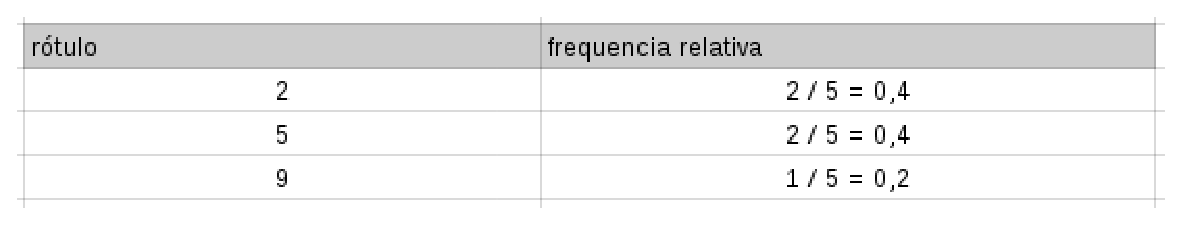
\includegraphics[width=0.9\textwidth]{figuras/frequencia_relativa.eps}
  \caption{Frequência relativa dos rótulos do treinamento}
  \label{fig:frequencia_relativa}
\end{figure}

Cada parâmetro condicional $\hat{P}(x_i | c)$ é um peso que representa a qualidade
do atributo $x_i$ como indicador da classe c. No exemplo, $x_i$ representa uma
posiçao no vetor de pixels, ou seja, o valor do pixel na posição i, onde essa
probabilidade pode ser calculada através da seguinte fórmula.

\begin{center}

$ \hat{P}(x_i | c) \ = \ \frac{T_{cx} + 1}{\sum\limits_{x' \in V}T_{cx'} + 1} $
\\
\end{center}

``Onde $T_{cx}$ é o número de ocorrências de x em objetos de exemplo da classe c''
\citeonline{araujo2011apprecommender}, no exemplo, $T_{cx}$ é a quantidade de
ocorrências de um valor do pixel, que é o x, para um dado rótulo, definido pela
variavel c, logo o utilizando o vetor de entrada mostrado na figura~\ref{fig:bayes_dado_entrada_convertida},
o valor de T, onde a classe c é o rótulo 2 para o primeiro pixel dos dados dados
de entrada de entrada da figura~\ref{fig:bayes_dado_entrada_convertida} é 2, pois
há dois rótulos de valor dois que o primeiro pixel é o valor zero, a figura~\ref{fig:tcx_dos_rotulos}
mostra os valores $T_{cx}$ utilizando os dados de entrada da figura~\ref{fig:bayes_dado_entrada_convertida}.

\begin{figure}[h]
  \centering
  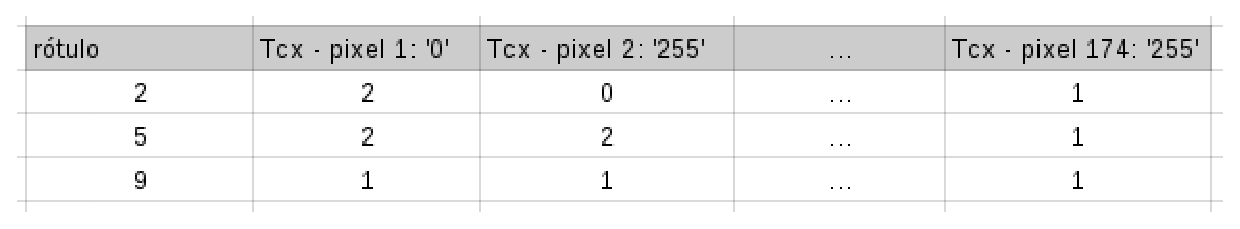
\includegraphics[width=0.9\textwidth]{figuras/tcx_dos_rotulos.eps}
  \caption{Tcx dos rótulos}
  \label{fig:tcx_dos_rotulos}
\end{figure}

O valor V é o conjunto dos atributos que uma classe c possui, logo, no exemplo
do reconhecimento de dígito na imagem, V é um conjunto que possui dois valores
0 e 255, sendo assim, a somatória ``$\sum\limits_{x' \in V}T_{cx'}$'' é igual a
quantidade de rótulos c nos dados de treinamento da figura~\ref{fig:tabela_ml_treinamento_convertida},
no caso, a somatória ``$\sum\limits_{x' \in V}T_{cx'}$'' para o rótulo 2 é igual
a dois, pois há dois rótulos 2, a figura~\ref{fig:somatoria_tcx_dos_rotulos}
mostra a somatória ``$\sum\limits_{x' \in V}T_{cx'}$'' para todos os rótulos dos
dados de treinamento para os dados de entrada da figura~\ref{fig:bayes_dado_entrada_convertida}.

\begin{figure}[h]
  \centering
  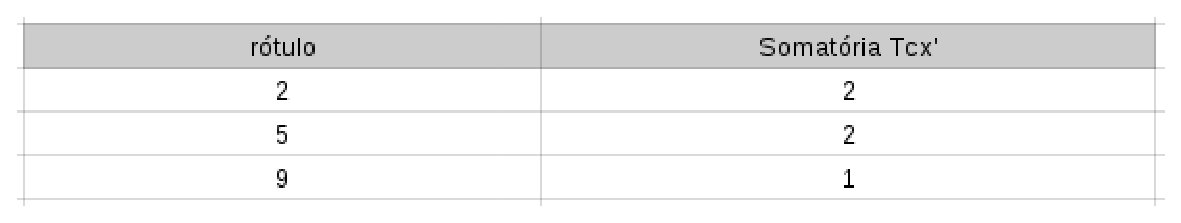
\includegraphics[width=0.9\textwidth]{figuras/somatoria_tcx_dos_rotulos.eps}
  \caption{Tcx dos rótulos}
  \label{fig:somatoria_tcx_dos_rotulos}
\end{figure}

Utilizando os dados da figura~\ref{fig:tcx_dos_rotulos} e da figura~\ref{fig:somatoria_tcx_dos_rotulos}
se realiza os calculos de probabilidade para os dados de entrada da
figura~\ref{fig:bayes_dado_entrada_convertida}, onde está demonstrado apenas para
os pixels 1, 2 e 784 da imagem, que são mostrados na figura~\ref{fig:probabilidades_dos_rotulos},
onde o rótulo de maior probabilidade usando esses três pixels é o rótulo X, o
correto é aplicar o cáculo a todos os pixels, porém, por se tratar de um exemplo
optou-se por aplicar apenas a esses três pixels, o 1, 2 e 784.

\begin{figure}[h]
  \centering
  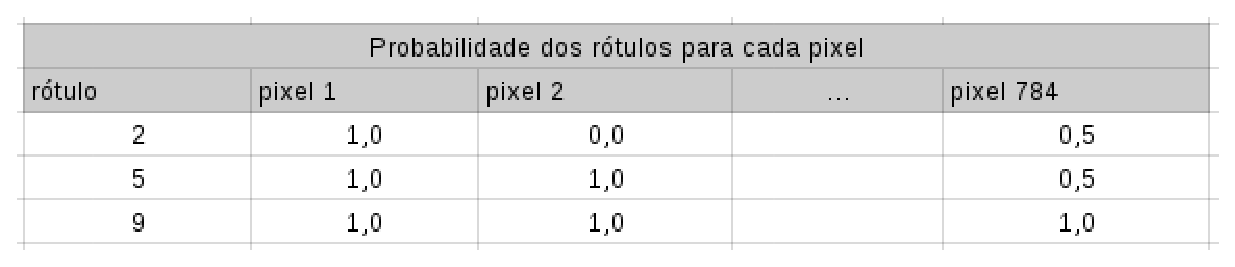
\includegraphics[width=0.9\textwidth]{figuras/probabilidades_dos_rotulos.eps}
  \caption{Probabilidade dos rótulos para cada pixel}
  \label{fig:probabilidades_dos_rotulos}
\end{figure}

Através dessa demonstração e considerando apenas os três pixels, 1, 2 e 784,
para a entrada de dados da figura~\ref{fig:bayes_dado_entrada_convertida}, o
algoritmo responderá que o numéro na imagem é o X.
